\documentclass[12pt]{exam}

\usepackage{fullpage, amsmath, amssymb, amsthm}
\usepackage{tikz} 

\renewcommand{\partshook}{\setlength\itemsep{1em}}
\newcommand{\D}{\displaystyle}
\newcommand{\CC}{\mathbb{C}}
\newcommand{\RR}{\mathbb{R}}
\newcommand{\dd}{\mathrm{d}}
\newcommand{\dz}{\mathrm{d}z}
\newcommand{\dx}{\mathrm{d}x}

\newcommand{\cic}{\frac1{2\pi i}\int_C}
\renewcommand{\epsilon}{\varepsilon}
\renewcommand{\Re}{\operatorname{Re}}
\renewcommand{\Im}{\operatorname{Im}}
\DeclareMathOperator{\Log}{Log}
\DeclareMathOperator{\Arg}{Arg}
\DeclareMathOperator{\sign}{sign}
\DeclareMathOperator{\length}{length}


\begin{document}

\section*{MATH 307 --- Worksheet \#5 }

\begin{questions}
    \setlength\itemsep{1em}
    \setlength\parskip{1em}

    
    \question
    
    Compute the integral. All curves are oriented counterclockwise.

    \bigskip
    \begin{parts}
        \item $\D\cic \frac{z\cos z}{(z+2i)^2}\dz$, where $C$ is the unit circle
        
        \begin{solution}
            The integrand is analytic on and inside the simple, closed curve $C$. Therefore,
            $$\cic \frac{z\cos z}{(z+2i)^2}\dz=0.$$
        \end{solution}

        \item $\D\cic \frac{z\cos z}{z-2i}\dz$, where $C$ is the circle $|z-i|=2$

        \begin{solution}
            The function $e^{2z}$ is analytic on and inside $C$.
            Since $2i$ lies inside $C$,
            $$\cic \frac{z\cos z}{z-2i}\dz = e^{2i},$$
            by Cauchy's integral formula.
        \end{solution}

        \item $\D\cic \frac{2e^{2z}}{z^2+1}\dz$, where $C$ is the square with vertices at $1$, $1+2i$, $-1+2i$, and $-1$.
        
        \begin{solution}
        Do a partial fraction decomposition:
        \[
            \frac{2}{z^2+1} = \frac1{(z-i)(z+i)} = -\frac i{z-i} + \frac i{z+i}
        \]
        Then
        $$\cic \frac{2e^{2z}}{z^2+1}\dz
        = -\cic\frac{i  e^{2z}}{z-i}\dz + \cic\frac{i  e^{2z}}{z+i}\dz$$
        By Cauchy's integral formula,
        $$
        \cic\frac{i  e^{2z}}{z-i}\dz = i e^{2i}.
        $$
        Since $\D\frac{i  e^{2z}}{z+i}$ is analytic on and inside $C$, 
        $$
        \int_C\frac{i  e^{2z}}{z+i}\dz=0,
        $$
        by Cauchy's theorem.
        Therefore,
        $$
        \cic \frac{2e^{2z}}{z^2+1}\dz = -i e^{2i}.
        $$
        \end{solution}
        
        \item $\D\cic \frac{2ze^z}{z^2+1}\dz$, where $C$ is the circle $|z|=2$
        
        \begin{solution}
            Arguing as in the previous problem,
            $$\cic \frac{2ze^{2z}}{z^2+1}\dz
                = -\cic\frac{iz  e^{2z}}{z-i}\dz + \cic\frac{iz  e^{2z}}{z+i}\dz
            $$
            By two applications of Cauchy's integral formula,
            $$
            \cic \frac{2ze^{2z}}{z^2+1}\dz = -i^2e^{2i} + i^2e^{-2i} = e^{2i} - e^{-2i}.
            $$
        \end{solution}
        
        \item $\D\cic \frac{e^{3z}}{z^3}\dz$, where $C$ is the unit circle
        
        \begin{solution}
            By Cauchy's integral formula for derivatives,
            $$\cic \frac{e^{3z}}{z^3}\dz = \frac1{2!}\left.\frac{d^2}{dz^2}\right|_{z=0}e^{3z} = \frac92.
            $$
        \end{solution}
        
        \item $\D\cic \frac{e^{3z}}{z^3-2z^2}\dz$, where $C$ is the unit circle $|z|=2$
        
        \begin{solution}
            Do a partial fraction decomposition:
            $$
            \frac1{z^2} = -\frac1{z} - \frac1{z^2} + \frac1{z-1}
            $$
            Therefore,
            $$
                \cic \frac{e^{3z}}{z^3-2z^2}\dz = -\cic \frac{e^{3z}}{z}\dz
                - \cic \frac{e^{3z}}{z^2}\dz
                + \cic \frac{e^{3z}}{z-1}\dz.
            $$
            By three applications of Cauchy's integral formula, one involving the derivative,
            $$
            \cic \frac{e^{3z}}{z^3-2z^2}\dz = -e^{3(0)} - 3e^{3(0)} + e^{3(1)} = -4 + e^3.
            $$
        \end{solution}
    \end{parts}

    \question
    In this problem, we evaluate the real, improper integral
    $$
        I := \int_{-\infty}^\infty \frac\dx{(x^2+1)^2}.
    $$

    \bigskip
    \begin{parts}


    \part Let $R>0$. Use Cauchy's integral formula to compute
    \[
        J_R := \int_{\gamma_R}\frac{\dz}{(z^2+1)^2},
    \]
    where $\gamma_{R}$ is the simple, closed curve drawn in blue below.
    \begin{center}
    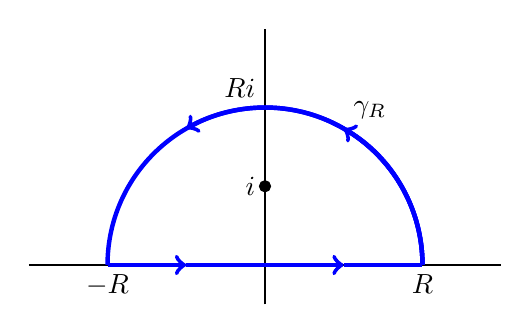
\begin{tikzpicture}
        \draw[thick] (-3, 0) -- (3, 0);
        \draw[thick] (0, -0.5) -- (0, 3);
        \draw[ultra thick, ->, blue] (2,0) arc (0:60:2);
        \draw[ultra thick, ->, blue] (2,0) arc (0:120:2);
        \draw[ultra thick, blue] (2,0) arc (0:180:2);
        \draw[ultra thick, ->, blue] (-2, 0) -- (-1, 0);
        \draw[ultra thick, ->, blue] (-1, 0) -- (1, 0);
        \draw[ultra thick, blue] (1, 0) -- (2, 0);
        \node at (1, 1.73) [above right] {$\gamma_R$};
        \node at (0, 2) [above left] {$Ri$};
        \node at (2, 0) [below] {$R$};
        \node at (-2, 0) [below] {$-R$};
        \node at (0, 1) [left] {$i$};
        \filldraw [black] (0,1) circle (2pt);
        \end{tikzpicture}
    \end{center}

    \begin{solution}
        Do a partial fraction decomposition:
        \begin{align*}
            \frac{1}{(z^2+1)^2} &= \frac{\dz}{(z-i)^2(z+i)^2}\\
            &= \frac14\left(\frac i{z+i} - \frac1{(z+i)^2}-\frac i{z-i} - \frac1{(z-i)^2}\right)
        \end{align*}
        Since $-i$ is outside $\gamma_R$,
        \begin{align*}
            J_R &= -\frac14\left(i\int_{\gamma_R}\frac{\dz}{z-i} + \frac{\dz}{(z-i)^2}\right)\\
            &= -\frac14(i(2\pi i) + 0)\\
            &= \frac\pi 2
        \end{align*}
        By two applications of Cauchy's integral formula,
        one for the value of $f(z)=1$ at $z=i$ and one for the derivative of $f(z)=1$ at $z=i$.
    \end{solution}

    \part Let $\delta_R$, be the semicircular portion of $\gamma_R$.
    Show that
    $$
    |K_R|\leq \frac{\pi R}{(R^2-1)^2},
    \qquad\text{where}\qquad
    K_R := \int_{\delta_R}\frac{\dz}{(z^2+1)^2}.
    $$
    Hint: Show that $|z^2+1|\geq R^2-1$ for $z$ on $\gamma_R$, then use the $ML$-bound.

    \begin{solution}
        If $z$ is on $\delta_R$, then $z^2$ is on the circle of radius $R^2$ centered at $0$
        and $z^2+1$ lies outside the circle with radius $R^2-1$ centered at $0$.
        Therefore, $|z^2+1|\geq R^2-1$ and
        \[
            \frac1{|z^2+1|^2}\leq \frac1{(R^2-1)^2}.
        \]
        Therefore, by the $ML$-bound, 
        \begin{align*}
            \left|\int_{\delta_R}\frac{\dz}{(z^2+1)^2}\right| \leq \frac{\pi R}{(R^2-1)^2}.
        \end{align*}
    \end{solution}

    \part Briefly justify the identity
    \[
        J_R = K_R + I_R,\qquad\text{where}\qquad I_R := \int_{-R}^R\frac{\dx}{(x^2+1)^2}.
    \]
    Let $R\to\infty$ and evaluate $I$.

    \begin{solution}
        $J_R=K_R+I_R$ by path additivity of line integrals. Therefore,
        \begin{align*}
            I &= \lim_{R\to\infty} I_R\\
            &= \lim_{R\to\infty}(J_R - K_R)\\
            &= \frac\pi 2 - \lim_{R\to\infty} K_R\\
            &=\frac\pi 2,
        \end{align*}
        since $K_R\to 0$ as $R\to\infty$ by (b).
    \end{solution}
\end{parts}
\end{questions}
\end{document}